En el presente trabajo se va a describir la \trabajo. Se comenzará dando una definición y repasando sus orígenes y evolución. Se introducirá la terminología asociada a este modelo. A continuación, se definirán los conceptos más relevantes, así como las herramientas usadas para cumplir con este modelo. Por último, se extraerán unas conclusiones de todo el trabajo realizado.

\section{Definición}

De acuerdo con la página oficial del instituto CMMI, la \trabajo o \textit{CMMI}\footnote{Siglas del nombre en inglés Capability Maturity Model Integration} es un ``conjunto probado de buenas prácticas globales que conducen el rendimiento del negocio a través de construir y analizar las capacidades clave'' \cite{definition}. Dicho con otras palabras, el CMMI es un modelo que permite a las organizaciones la promoción de comportamientos que ayuden a minimizar los riesgos durante el desarrollo de un producto o servicio. Una característica importante de CMMI es que es un marco de trabajo, es decir, indica qué se debe hacer, no cómo hacerlo \cite{definition2}\cite{definicion3}.

\section{Orígenes y evolución}

El CMMI fue creado por el Instituto de Ingeniería del Software (\textit{Software Engineering Institute o SEI}) que estaba patrocinado por el Departamento de Defensa de los Estados Unidos de América. Su objetivo original era evaluar tanto la capacidad como la calidad de sus servicios software. Con el tiempo, este modelo trascendió las fronteras del software para ser utilizado en cualquier tipo de industria, con el fin de medir y mejorar sus capacidades, y así mejorar su rendimiento. Actualmente, CMMI está administrado por el Instituto CMMI, que fue comprado por \textit{ISACA} en 2016 \cite{definition}\cite{definition2}.\\

El CMMI fue desarrollado para integrar múltiples modelos de madurez empresarial en un único marco de trabajo. A lo largo de los años, han existido varias versiones de CMMI, las cuales se irán describiendo en las siguientes líneas \cite{history}: 

\begin{itemize}
    \item \textbf{CMMI v1.1.} Desde que surgieron los primeros computadores, los proyectos software que se llevaban a cabo eran principalmente amateur, por lo que solían tener muchos fallos. No fue hasta los años 80, cuando el Departamento de Defensa de los Estados Unidos de América intervino. Esta intervención fue debida a que los proyectos militares que involucraban software subcontratado se retrasaban debido al software, precisamente. Como consecuencia, el ejército de EEUU financió un estudio en el ya mencionado SEI para determinar las causas de los constantes retrasos del software. Entre tanto, un hombre llamado Watts Humphrey había empezado a desarrollar un proyecto que iba en la misma línea que lo que el ejército quería. Dicho modelo estaba basado en \textit{``The Quality Management Maturity Grid''} o \textit{QMMG}\footnote{QMMG es una matriz de madurez organizacional usada por las empresas para evaluar la madurez de sus procesos. Fue desarrollada en 1979 por Philip B. Crosby.}. Cuando Hymphrey se unió al SEI fue capaz de formalizar el trabajo que había realizado hasta ahora, dando lugar a un Modelo de Madurez de Capacidades (CMM) que fue publicado en 1988, y en 1989 en forma de libro \footnote{Bajo el título de \textit{Managing the Software Process.}}. Mas tarde, el SEI formalizaría los conceptos propuestos en ese modelo dando lugar al Modelo de Madurez de Capacidades para Software o \textit{SW-CMM}. La versión 1.0 de este modelo se publicó en 1991, y dos años más tarde lo haría la versión 1.1 (en 1995, en forma de libro).\\
    
    Tras el lanzamiento de la versión para software, surgieron otros modelos de madurez de capacidades para otras industrias, como la ingeniería de sistemas (SE-CMM), la adquisición de software, el desarrollo de productos integrados, etc. De hecho, cuando la versión 2.0 del SW-CMM iba a ser lanzada en 1997, esta se canceló en favor de un proyecto que integrada los múltiples modelos que habían nacido para las diferentes industrias y negocios. Este proyecto era el CMM Integration o CMMI. Dicho proyecto era una colaboración conjunta del gobierno, la industria y el SEI y dio lugar, en 2002, al CMMI v1.1. 
    
    \item \textbf{CMMI v1.2.} Tras el lanzamiento de CMMI v1.1, se lanzaría el CMMI v1.2 en el año 2006, añadiéndose nuevos ejemplos y consolidando y simplificando las prácticas \textit{IPPD}\footnote{\textit{Integrated Product and Process Development}.}. Esta versión 1.2 añadió, además, el concepto de \textit{constelaciones}, que hace referencia a un conjunto de componentes diseñados para satisfacer las necesidades de un área de interés específica. Así, surgieron tres constelaciones: una para el desarrollo (\textit{Dev}), una para los servicios (\textit{SVC}) y otra para la adquisición (\textit{ACQ}) \cite{cmmmiv12}.
    
    \item \textbf{CMMI v1.3.} En el año 2010 se lanzó CMMI v1.3, que añadió características como el soporte para desarrollo ágil de software, además de consolidar los modelos para las tres áreas de interés principales: desarrollo, servicios y adquisición. 
    
    \item \textbf{CMII v2.0.} En el año 2018 se lanzaría la versión 2.0, que es la más reciente publicada. En esta versión, se incluyen cambios importantes, tal como la integración de las tres constelaciones antes mencionadas en un solo modelo, de tal manera que se propongan una serie de prácticas comunes a todas ellas, y luego otra serie de prácticas más específicas. Esta versión añade además otra serie de cambios con respecto a la versión anterior, ya que v2.0 está más centrado en el rendimiento, tiene una mejor usabilidad y es más fácil de entender y de ser accedido \cite{history2}\cite{13vs20}.
\end{itemize}

En la Figura \ref{fig:evolution} se muestra un diagrama de la evolución del CMMI hasta la versión 1.3.

\begin{figure}[h]
    \centering
    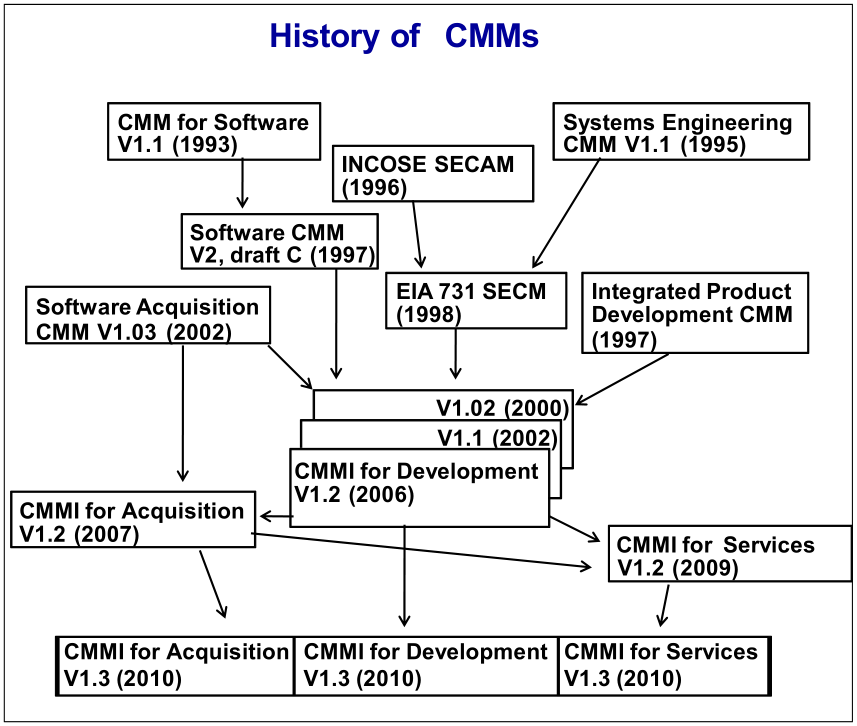
\includegraphics[width=\textwidth]{Images/evolution.PNG}
    \caption{Evolución del CMMI hasta la versión 1.3}
    \label{fig:evolution}
\end{figure}
